\chapter{Resultados}
En esta sección se presentan los resultados de la caracterización del voltaje de ruptura, ganancia, conteo oscuro, \textit{crosstalk} y \textit{afterpulses} en función de la temperatura y del sobre-voltaje, para los SiPMs S13360-1350CS de Hamamatsu y CPTA 151.   
\label{Cap:Caracterizacion}
\section{Sensores estudiados.}
Los módulos electrónicos desarrollados en este trabajo se utilizaron para caracterizar los principales parámetros de rendimiento de SiPMs en general. En este caso se eligieron dos SiPM a caracterizar: el SiPM S13360-1350CS y el CPTA 151.
\begin{figure}[h!]
\begin{centering}
  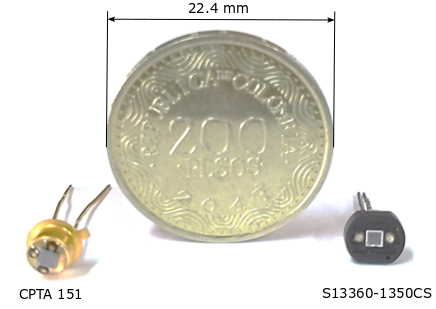
\includegraphics[width=0.5\textwidth]{Images/SiPMs.PNG}
    \caption{Fotomultiplicadores de silicio, en la parte izquierda el CPTA 151, en la derecha el Hamamatsu S13360-1350CS.}% junto a una moneda de 200 pesos colombianos.}
    \label{fig:SiPMs}  
  \par\end{centering}
\end{figure}
\\ \\
El SiPM de la serie S13360-1350CS de Hamamatsu %tilizado en el proyecto MuTe, donde se registra el flujo del componente muónico de rayos cósmicos secundarios (CRs) que pasan a través de formaciones geológicas para obtener imágenes de su estructura interna en función de sus diferencias de densidad \citep{minimute,Mute_oficial}.\\ 
utilizado para mediciones de precisión, hereda las excelentes características de bajo \textit{afterpuse} de series anteriores, además de proporcionar menor \textit{crosstalk} y \textit{dark count}.
El SiPM CPTA 151 utilizado para el desarrollo de prototipos para tomografía computarizada de protones, en el Laboratorio Nacional Fermi (Fermilab) \citep{pCT_fermilab}.\\ \\% donde se utilizan estos SiPMs para detectar los fotones generados por fibras centelladoras al paso de partículas cargadas, lo que permite hacer un rastreo de la partícula con una alta resolución espacial \citep{pCT_fermilab}.\\  
%Para el estudio de los SiPMs es de especial interés los parámetros de rendimiento. En esta sección se abordan los más relevantes, se muestra su comportamiento teórico y se presentan algunas gráficas del comportamiento de estos parámetros en el SiPM S133360-1350CS. 
En la Tabla \ref{table_SiPMs} se muestran los principales parámetros de rendimiento suministrados por el fabricante para cada uno de los sensores estudiados. %Particularmente, para el SiPM CPTA 151 el fabricante no suministra suficiente información, por lo tanto su caracterización toma aún más importancia.  
\begin{table}[h!]
\caption{Parámetros de los sensores estudiados. Adaptado de \citep{Sipm_S13360_1350CS_datasheet, CPTA_data}.}
    \label{table_SiPMs}
%	\centering
	\begin{tabular}{ c  c  c}
    \hline
    Parámetro                                                   & S13360-1350CS (T=25$^\circ$C)     & CPTA 151 (T=22$^\circ$C)  \\ \hline
    \multicolumn{1}{l}{Número de píxeles}                       & $667$              & $796$       \\
    \multicolumn{1}{l}{Tamaño del píxel ($\mu m^2$)}               & $50\mbox{x}50$               & $40\mbox{x}40$       \\
    \multicolumn{1}{l}{\´Área fotosensible ($\mbox{mm}^2$)}     & $1.3\times1.3$     & $1.28\times1.28$\\
  %  \multicolumn{1}{l}{Factor de llenado (\%)}                  & $74$               & $---$       \\
    \multicolumn{1}{l}{Pico de sensitividad (nm)}               & $450$              & $600$       \\
    \multicolumn{1}{l}{Ganancia}                                & $1.7\times10^6$    & $4\times10^5$       \\
    \multicolumn{1}{l}{DCR típica (kHz)}      & $90$               & $600$       \\
    \multicolumn{1}{l}{Probabilidad de \textit{crosstalk} (\%)} & $3$                & $10$       \\ \hline
	\end{tabular}
\end{table}
\section{Voltaje de ruptura}
El primer conjunto de mediciones, para visualizar la dependencia de la temperatura en el voltaje de ruptura, son las curvas de corriente contra voltaje (I-V) mostradas en la Fig. \ref{fig:dc} y obtenidas mediante un \textit{script} en Python \footnote{https://github.com/juanvillafrades/Caracterizacion-SiPMs/blob/master/BreakdownV.ipynb}. Estas curvas se obtienen realizando la medición de la corriente oscura (\textit{Dark current}) en los SiPM, para voltajes de operación ($V_{Bias}$) en el rango de 40 V a 60 V en el caso del SiPM de Hamamatsu y de entre 40 a 50 V para el caso del CPTA teniendo en cuenta los valores máximos recomendados por el fabricante. Estas curvas I-V se generan para temperaturas en el rango de 0 a 40 $^\circ$C, todo esto utilizando la configuración experimental mostrada en la Fig. \ref{fig:complete_system}.
\begin{figure}[h!]
     \centering
     \begin{subfigure}[b]{0.49\textwidth}
         \centering
         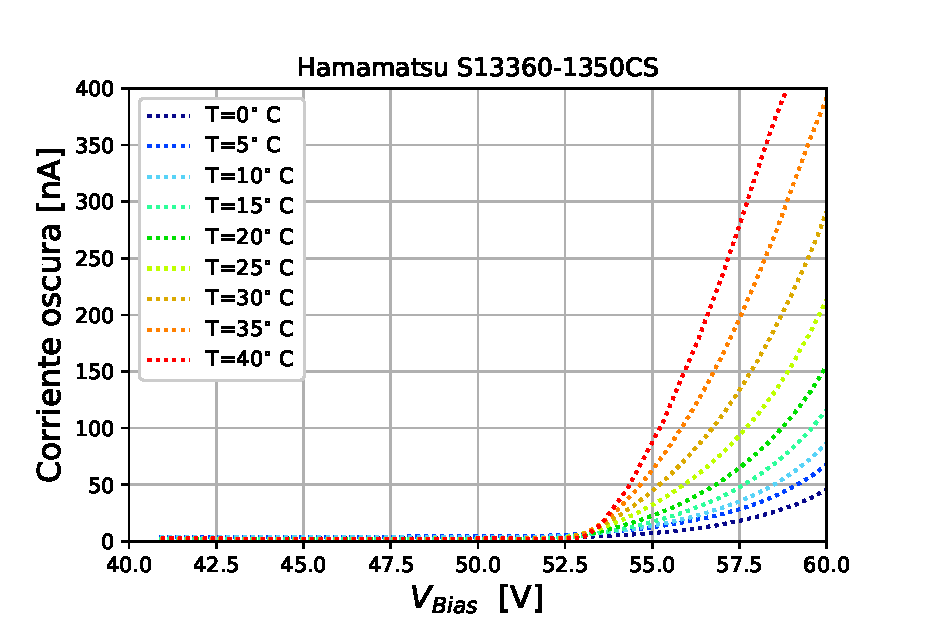
\includegraphics[width=1.1\textwidth]{Images/dc_13360.eps}
         \caption{}
         \label{fig:dc_13360}
     \end{subfigure}
     %\hfill
     \begin{subfigure}[b]{0.49\textwidth}
         \centering
         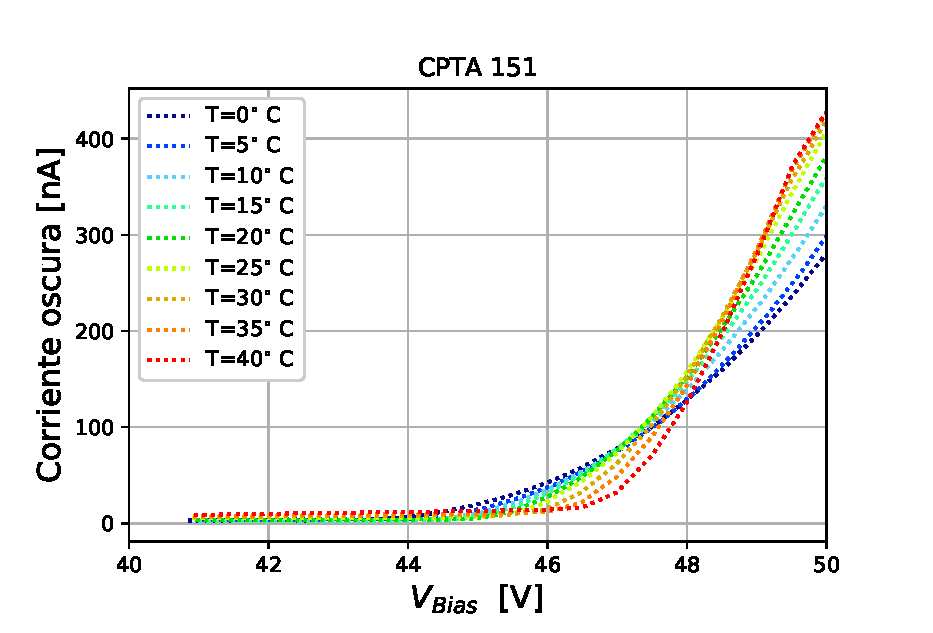
\includegraphics[width=1.1\textwidth]{Images/dc_CPTA.eps}
         \caption{}
         \label{fig:dc_cpta}
     \end{subfigure}
        \caption{Corriente oscura en función del voltaje de polarización para los sensores S13360-1350CS de Hamamatsu (izquierda) y CPTA 151 (derecha) en el rango de temperatura de $0~\mbox{a}~40~^\circ$C.}
        \label{fig:dc}
\end{figure}
\\ \\
En la Fig. \ref{fig:dc}. se observa un aumento en la pendiente de las curvas I-V a medida que la temperatura aumenta. Adicionalmente, se puede notar que las curvas I-V en la Fig. \ref{fig:dc}(a) tienen una menor dependencia de la temperatura, mientras que las curvas I-V en la Fig. \ref{fig:dc}(b) presentan una mayor dependencia para el rango de voltaje de polarización utilizado en cada sensor.
\\ \\
A partir de las curvas I-V se obtienen las curvas $log(I)~vs~V$, su punto de inflexión determina el voltaje de ruptura y se calcula como la intersección de la recta tangente a la curva  $log(I)$ y la línea base \citep{MPPC_note, Ruptura_metodo}. Este procedimiento se realiza para cada temperatura en el rango de análisis, en la Fig. \ref{fig:ruptura} se expone el procedimiento para una temperatura de 25 $^\circ$C.
\begin{figure}[h!]
\begin{centering}
  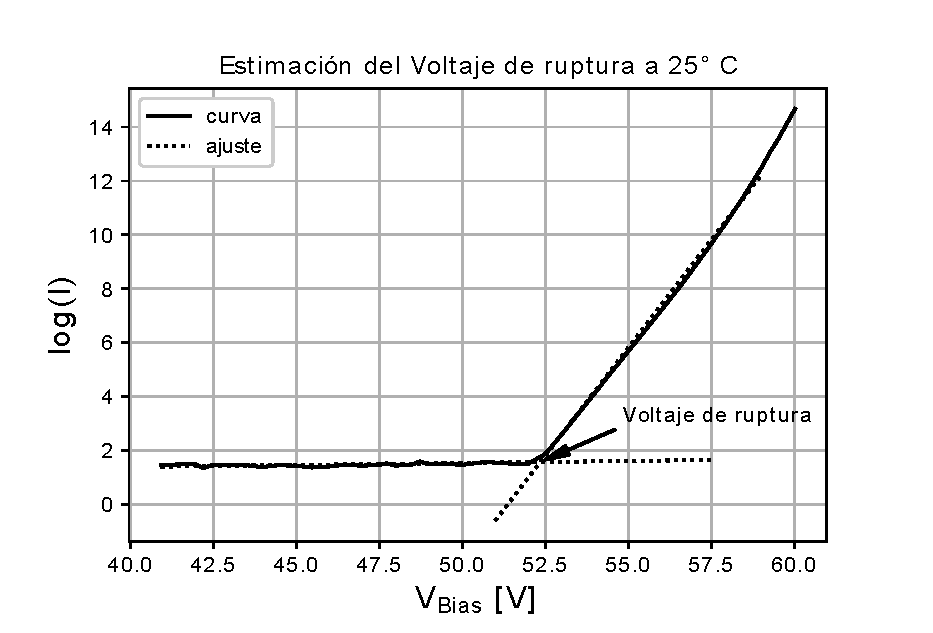
\includegraphics[width=0.6\textwidth]{Images/cal_voltaje_ruptura.eps}
  \caption{Método para la estimación del voltaje de ruptura, se muestra como ejemplo una temperatura de 25 $^\circ$C para el SiPM S13360-1350CS de Hamamatsu.}
  \label{fig:ruptura}
  \par\end{centering}
\end{figure}
\\
En la Fig. \ref{fig:Vbd_vs_T} se puede observar la curva de la dependencia de la temperatura para el voltaje de ruptura. Las funciones de ajuste para el SiPM S13360-1350CS de Hamamatsu ($V_{BD_{H}}$) y para el CPTA 151 ($V_{BD_{C}}$) son:
\begin{eqnarray}
V_{BD_{H}}(T) &=& 41.7\times10^{-3}[V/^\circ C]~T + 51.2~[V],\\
V_{BD_{C}}(T) &=& 66.5\times10^{-3}[V/^\circ C]~T+ 43.8~[V].
\end{eqnarray}
\begin{figure}[h!]
     \centering
     \begin{subfigure}[b]{0.49\textwidth}
         \centering
         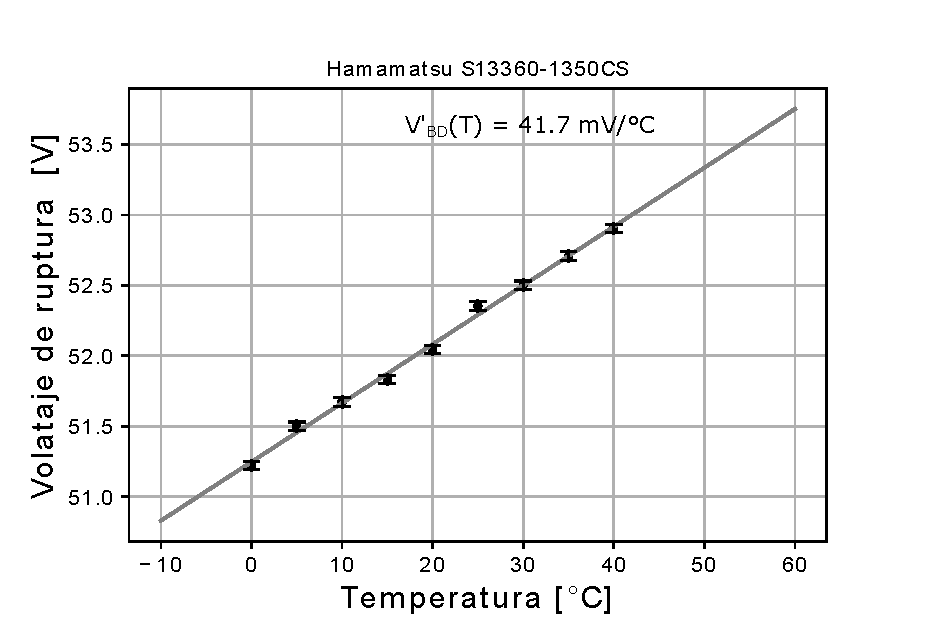
\includegraphics[width=1.1\textwidth]{Images/Vbd_vs_T_S13360.eps}
         \caption{}
         \label{fig:V_vd_13360}
     \end{subfigure}
     %\hfill
     \begin{subfigure}[b]{0.49\textwidth}
         \centering
         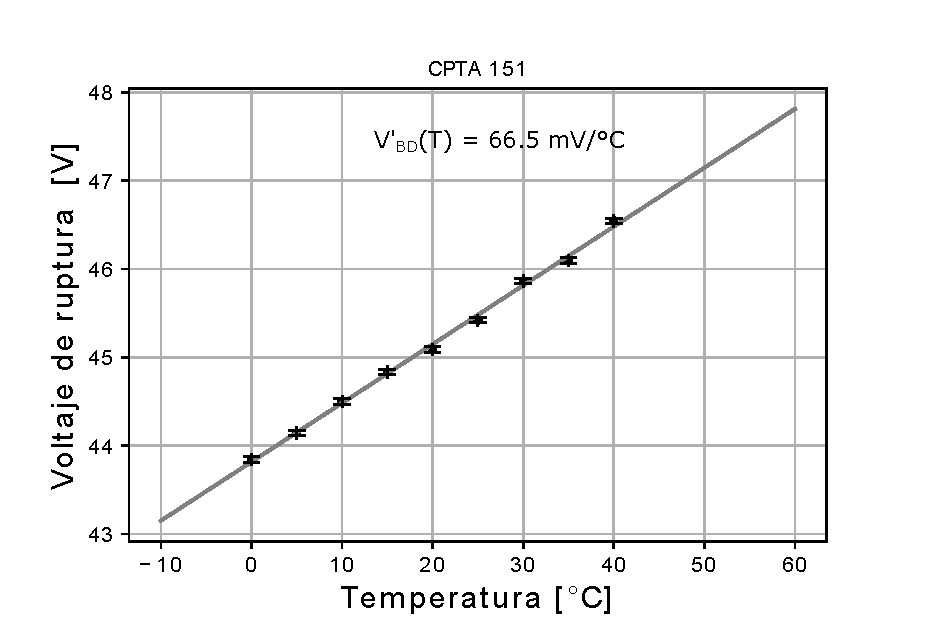
\includegraphics[width=1.1\textwidth]{Images/Vbd_vs_T_CPTA151.eps}
         \caption{}
         \label{fig:V_vd_cpta}
     \end{subfigure}
        \caption{Dependencia de la temperatura para el voltaje de ruptura en los SiPM S13360-1350CS de Hamamatsu (izquierda) y CPTA 151 (derecha). Se ajustó una línea recta, cuya pendiente determina el coeficiente de temperatura para el voltaje de ruptura. Se obtuvo $41.7$ mV/$^\circ$C para el S13360-1350CS de Hamamatsu y $66.5$ mV/$^\circ$C para el CPTA 151.}
        \label{fig:Vbd_vs_T}
\end{figure}
\section{Ganancia}
%Por otra parte el histograma de  carga se obtiene utilizando la configuración experimental expuesta en la figura \ref{fig:Data_system}. 
El histograma de carga de un SiPM es una representación gráfica del comportamiento estadístico de la carga generada por sus eventos. En la Fig. \ref{fig:charge}. se observa que el histograma de carga se compone de picos característicos equidistantes relacionados con la cantidad de fotones equivalentes (p.e.), el primer pico (0 p.e.) corresponde al pedestal y no se tiene en cuenta para ninguno de los cálculos realizados. El histograma de  carga se obtiene utilizando la configuración experimental expuesta en la Fig. \ref{fig:Data_system} y a partir de la integración de los pulsos de corriente generados por el SiPM, como se muestra a continuación:
\begin{equation}
Q = \displaystyle\sum_{0}^{t} i(k) \Delta  t = \displaystyle\sum_{0}^{t} \frac{v(k)}{F_A R} \Delta  t, 
\end{equation}
donde, $F_A$ es el factor de amplificación y R es la resistencia utilizada para realizar la conversión de corriente a voltaje. A partir del histograma de carga, a una temperatura de 25 $^\circ$C, se obtiene el equivalente de carga de 1 p.e. como el promedio de las diferencias entre cada uno de los picos del histograma. Para el caso del SiPM de Hamamatsu y CPTA se obtuvo $Q_{1pe_H}=0.206 $ pC y $Q_{1pe_C}=0.175 $ pC respectivamente. De esta forma, a partir de este equivalente de carga la ganancia se calcula como:
\begin{equation}
G = \frac{Q_{1pe}}{e},\\
%G_H &=& \frac{0.206\times10^{-12}}{1.602\times10^{-19}}\\
%G_H &=&1.29\times10^6\\
%G_C &=&1.09\times10^6
\end{equation}
donde, \textit{e} es la carga del electrón ($1.6\times10^{-19}$ C). En este caso, para una temperatura de 25 $^\circ$C se obtuvo una ganancia de $1.29\times10^6$ y $1.09\times10^6$ para el SiPM de Hamamatsu y CPTA respectivamente.
\begin{figure}[h!]
     \centering
     \begin{subfigure}[b]{0.49\textwidth}
         \centering
         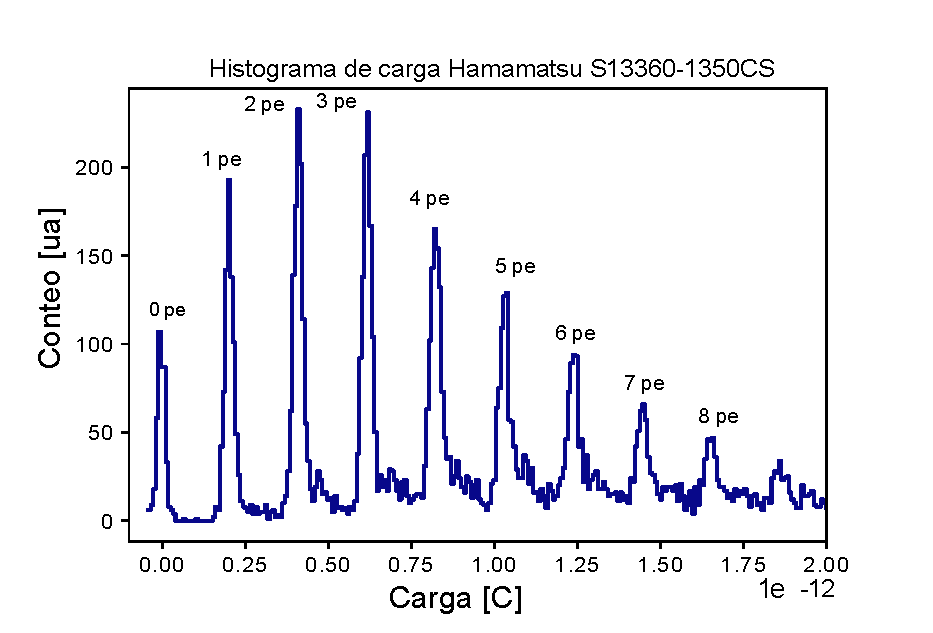
\includegraphics[width=1.1\textwidth]{Images/Charge_13360.eps}
         \caption{}
         \label{fig:charge_1360}
     \end{subfigure}
     %\hfill
     \begin{subfigure}[b]{0.49\textwidth}
         \centering
         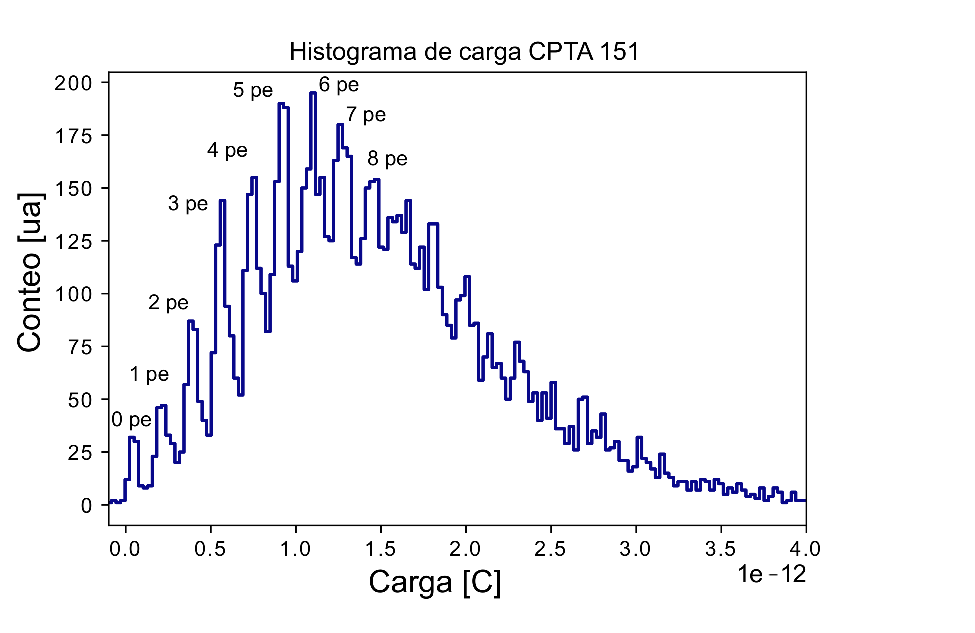
\includegraphics[width=1.1\textwidth]{Images/Charge_cpta.eps}
         \caption{}
         \label{fig:charge_cpta}
     \end{subfigure}
        \caption{Forma característica de los Histogramas de carga, el primer lóbulo corresponde al pedestal y los posteriores corresponden a múltiplos enteros de 1 p.e. Este histograma se obtuvo a una temperatura de 25 $^\circ$C.}
        \label{fig:charge}
\end{figure}
\\ \\
Para estudiar el comportamiento de la ganancia en función de la temperatura, se obtuvieron los histogramas de carga para cada una de las temperaturas de estudio, con un voltaje de polarización de 56 V para el SiPM S13360-1350CS de Hamamatsu y $53~\mbox{V}$ para el CPTA 151. En la Fig. \ref{fig:Gain_vs_T}. se muestra la relación inversamente proporcional entre la ganancia y la temperatura, con una dependencia de $-1.39\times 10^4/^\circ$C para el SiPM S13360-1350CS de Hamamatsu y $-1.22\times 10^4/^\circ$C para el  y CPTA 151.
% \begin{figure}[h!]
%      \centering
%      \begin{subfigure}[b]{0.49\textwidth}
%          \centering
%          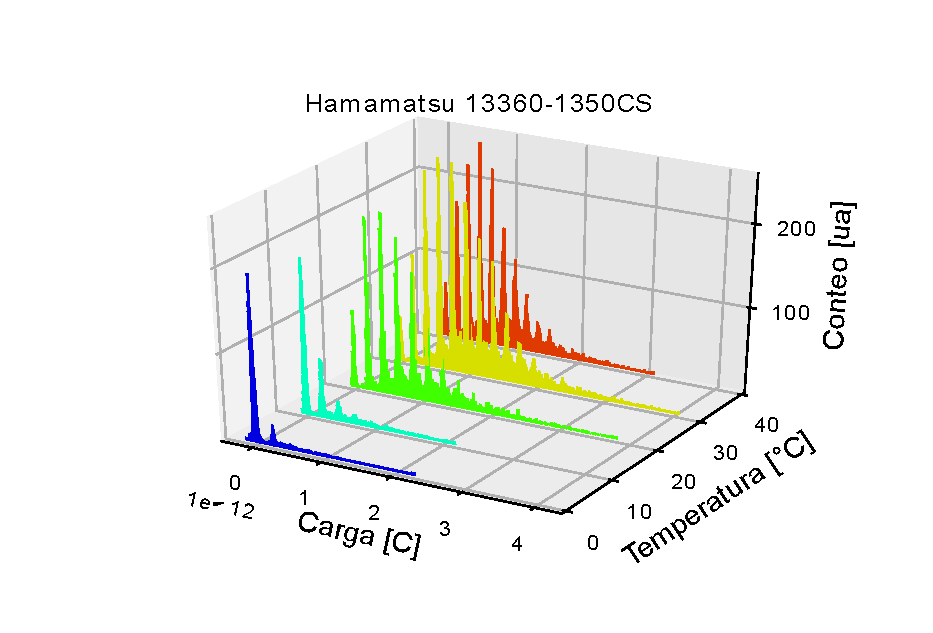
\includegraphics[width=1.1\textwidth]{Images/G_vs_T_1350CS.eps}
%          \caption{}
%          \label{fig:G_vs_T_1350CS}
%      \end{subfigure}
%      %\hfill
%      \begin{subfigure}[b]{0.49\textwidth}
%          \centering
%          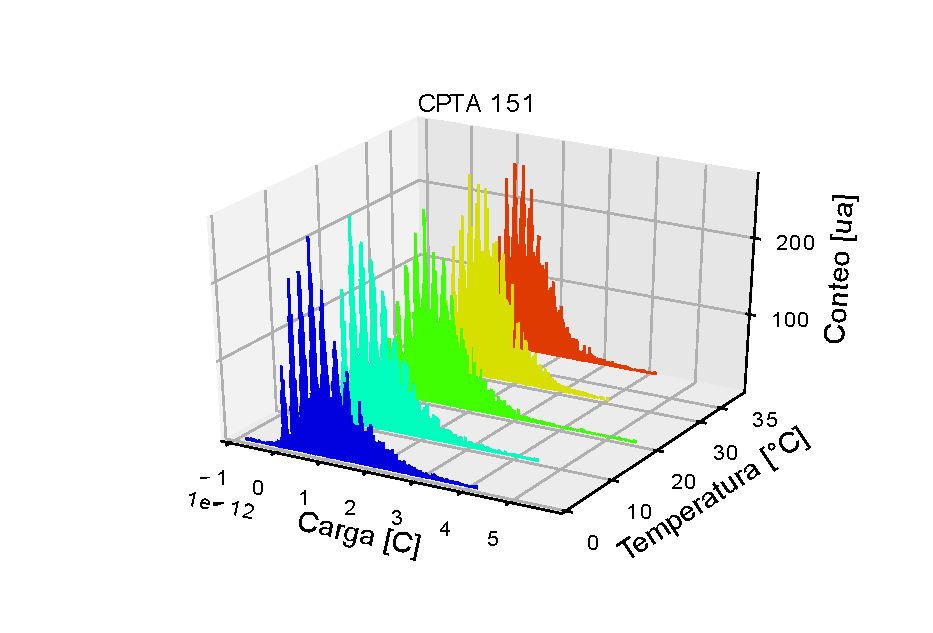
\includegraphics[width=1.1\textwidth]{Images/G_vs_T_CPTA151.eps}
%          \caption{}
%          \label{fig:G_vs_T_CPTA}
%      \end{subfigure}
%         \caption{Histogramas de carga a diferentes temperaturas entre 0 y 40 $^\circ$C. Donde se puede observar que la distancia entre los lóbulos del histograma aumentan a medida que la temperatura disminuye.}
%         \label{fig:His_G_vs_T}
% \end{figure}
\begin{figure}[h!]
     \centering
     \begin{subfigure}[b]{0.49\textwidth}
         \centering
         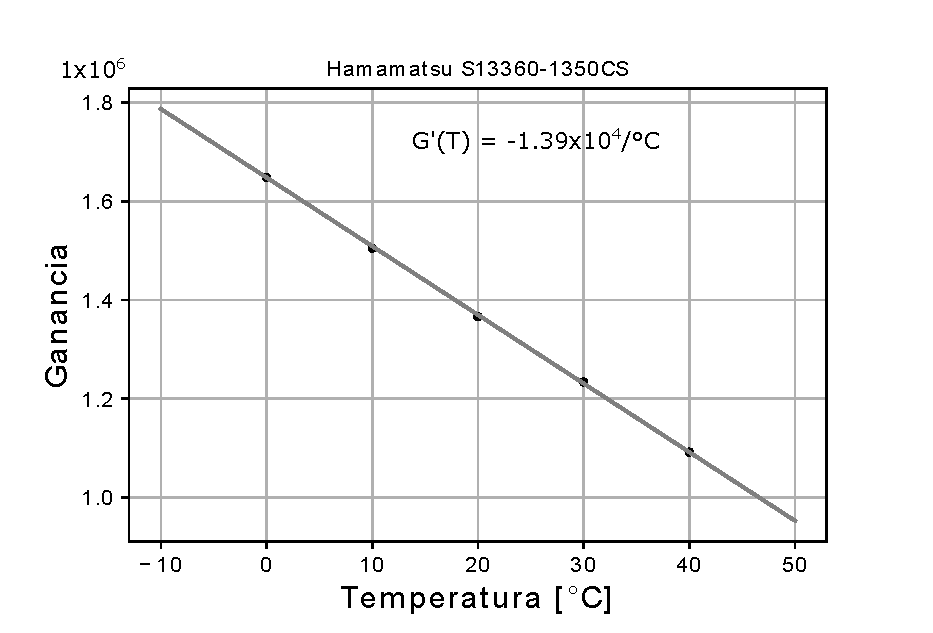
\includegraphics[width=1.1\textwidth]{Images/GT_1350CS.eps}
         \caption{}
         \label{fig:GT_1350CS}
     \end{subfigure}
     %\hfill
     \begin{subfigure}[b]{0.49\textwidth}
         \centering
         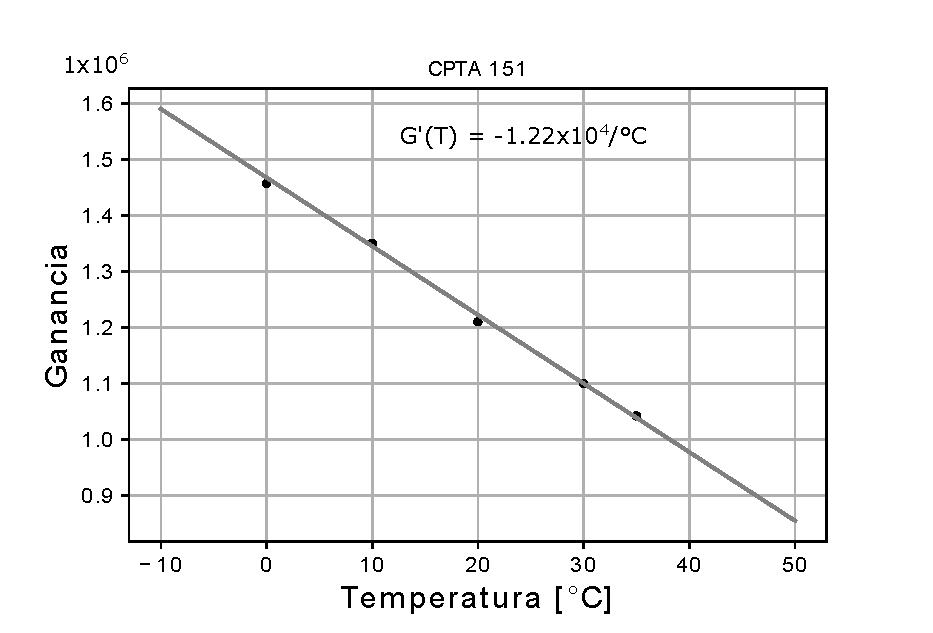
\includegraphics[width=1.1\textwidth]{Images/GT_CPTA.eps}
         \caption{}
         \label{fig:GT_CPTA}
     \end{subfigure}
        \caption{Ganancia en función de la temperatura para el SiPM S13360-1350CS de Hamamatsu (izquierda) y CPTA 151 (derecha). La pendiente de la linea recta ajustada a los datos representa el coeficiente de temperatura de la ganancia, siendo $-1.39\times10^4/^\circ$C para el SiPM S13360-1350CS de Hamamatsu y $-1.22\times10^4/^\circ$C para el CPTA 151.}
        \label{fig:Gain_vs_T}
\end{figure}
\\ \\
Por otra parte, se analizó el comportamiento de la ganancia en función del sobre-voltaje, para esto se estableció la temperatura a 25 $^\circ$C y se polarizaron los SiPM con tres valores de sobre-voltaje distintos, como se muestra en la Fig. \ref{fig:His_G_vs_ov}. La diferencia entre los picos del histograma (ganancia) aumenta a medida que el sobre-voltaje también lo hace, con una relación de $3.07\times10^5/V$ para el SiPM  S13360-1350CS de Hamamatsu y $1.65\times10^5/V$ para el CPTA 151 como se muestra en la Fig. \ref{fig:Gain_vs_ov}. 
\begin{figure}[h!]
     \centering
     \begin{subfigure}[b]{0.49\textwidth}
         \centering
         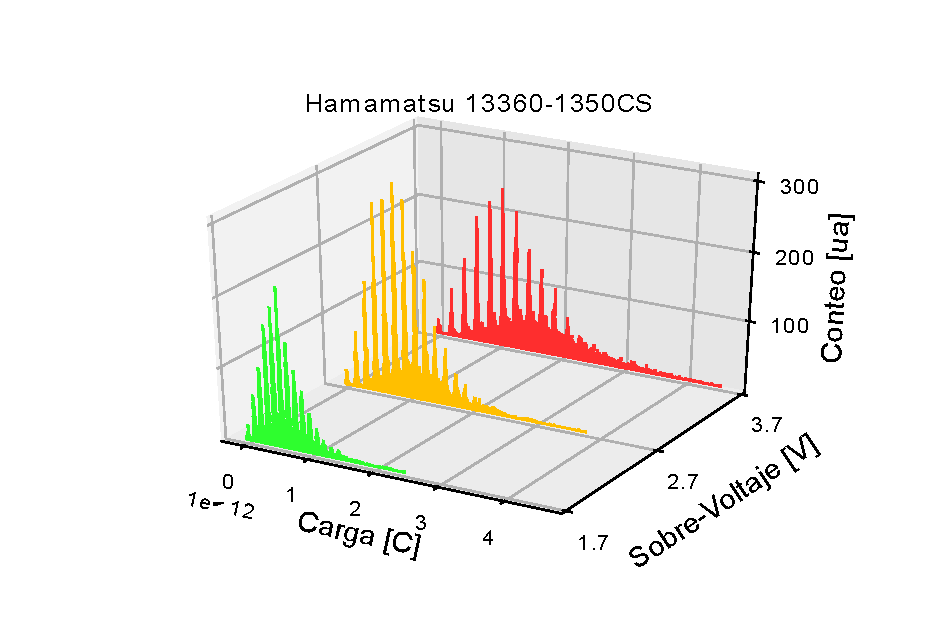
\includegraphics[width=1.1\textwidth]{Images/G_ov_1350CS.eps}
         \caption{}
         \label{fig:G_vs_ov_1350CS}
     \end{subfigure}
     %\hfill
     \begin{subfigure}[b]{0.49\textwidth}
         \centering
         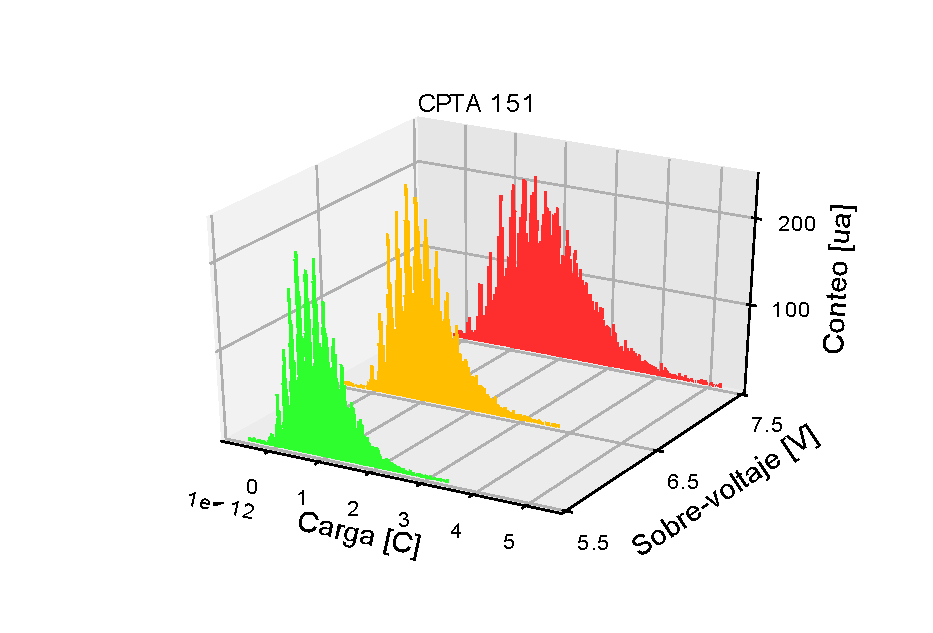
\includegraphics[width=1.1\textwidth]{Images/G_ov_CPTA151.eps}
         \caption{}
         \label{fig:G_vs_ov_CPTA}
     \end{subfigure}
        \caption{Histogramas de carga para tres valores de sobre-voltaje distintos a una temperatura de 25 $^\circ$C. La distancia entre los picos del histograma aumenta de forma directamente proporcional al valor del sobre-voltaje.}
        \label{fig:His_G_vs_ov}
\end{figure}
\begin{figure}[h!]
     \centering
     \begin{subfigure}[b]{0.49\textwidth}
         \centering
         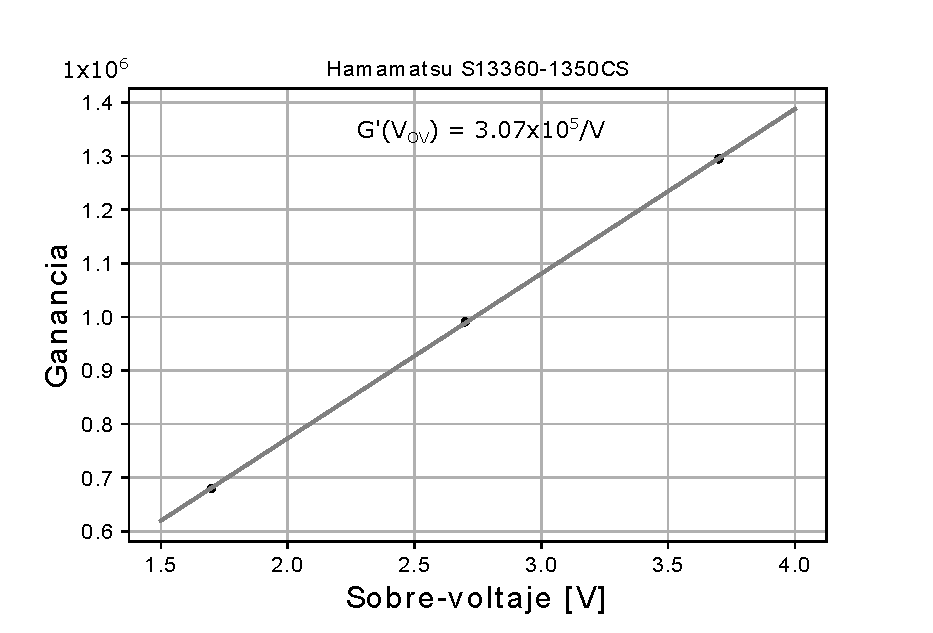
\includegraphics[width=1.1\textwidth]{Images/GOV_1350CS.eps}
         \caption{}
         \label{fig:Gov_1350CS}
     \end{subfigure}
     %\hfill
     \begin{subfigure}[b]{0.49\textwidth}
         \centering
         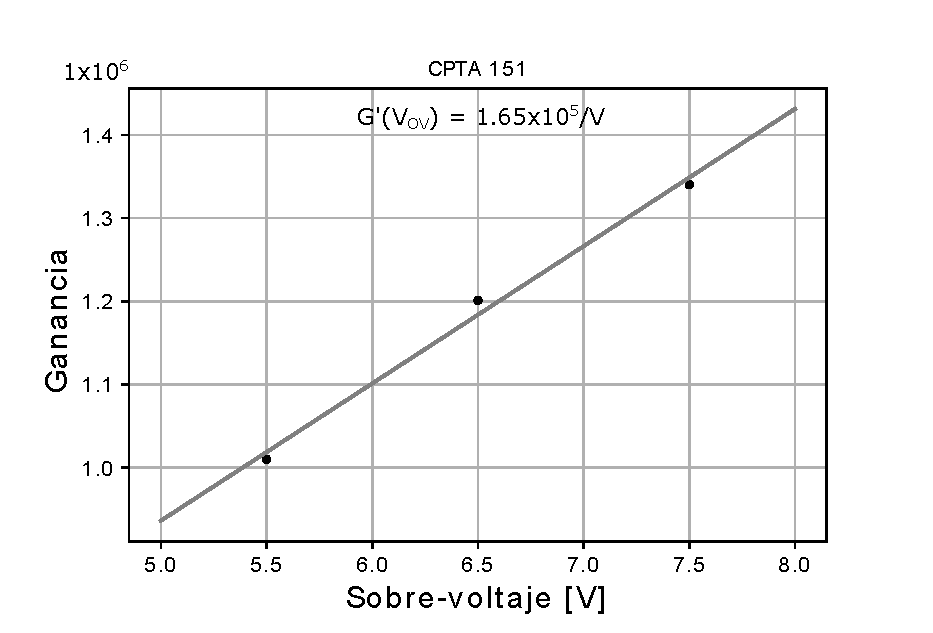
\includegraphics[width=1.1\textwidth]{Images/GOV_CPTA.eps}
         \caption{}
         \label{fig:Gov_CPTA}
     \end{subfigure}
        \caption{Dependencia del sobre-voltaje de la ganancia en los SiPM S13360-1350CS de Hamamatsu (izquierda) y CPTA 151 (derecha) a temperatura ambiente (25 $^\circ$C).}
        \label{fig:Gain_vs_ov}
\end{figure}
\section{Fotón equivalente}
En la sección anterior se calculó la carga de un fotón equivalente (p.e.), sin embargo, es necesario determinar el equivalente en voltaje de 1 p.e. para estimar los niveles de ruido. El histograma de pico de un SiPM es una representación estadística del valor máximo de los pulsos registrados, la diferencia promedio entre los picos de este histograma determina el equivalente de 1 p.e. como se muestra en la Fig. \ref{fig:peak}. En este caso para una temperatura de 25 $^\circ$C y unos voltajes de polarización de 56 V para el SiPM S13360-1350CS de Hamamatsu y 53 V para el  CPTA 151 un p.e. corresponde a $13.67~\mbox{mV}$ y $12.09~\mbox{mV}$ respectivamente.    
\begin{figure}[h!]
     \centering
     \begin{subfigure}[b]{0.49\textwidth}
         \centering
         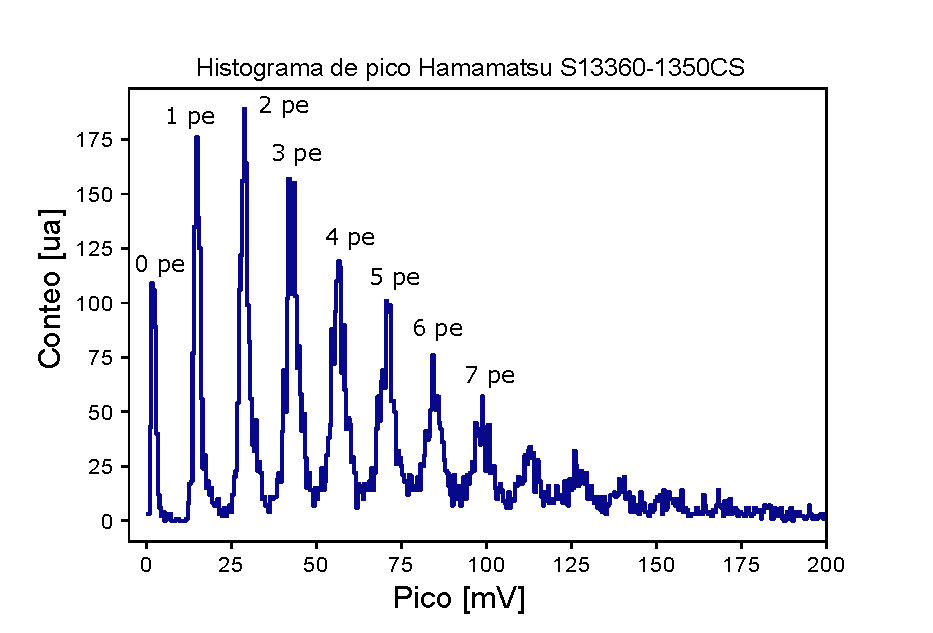
\includegraphics[width=1.1\textwidth]{Images/Peak_1350CS.eps}
         \caption{}
         \label{fig:peak_1350CS}
     \end{subfigure}
     %\hfill
     \begin{subfigure}[b]{0.49\textwidth}
         \centering
         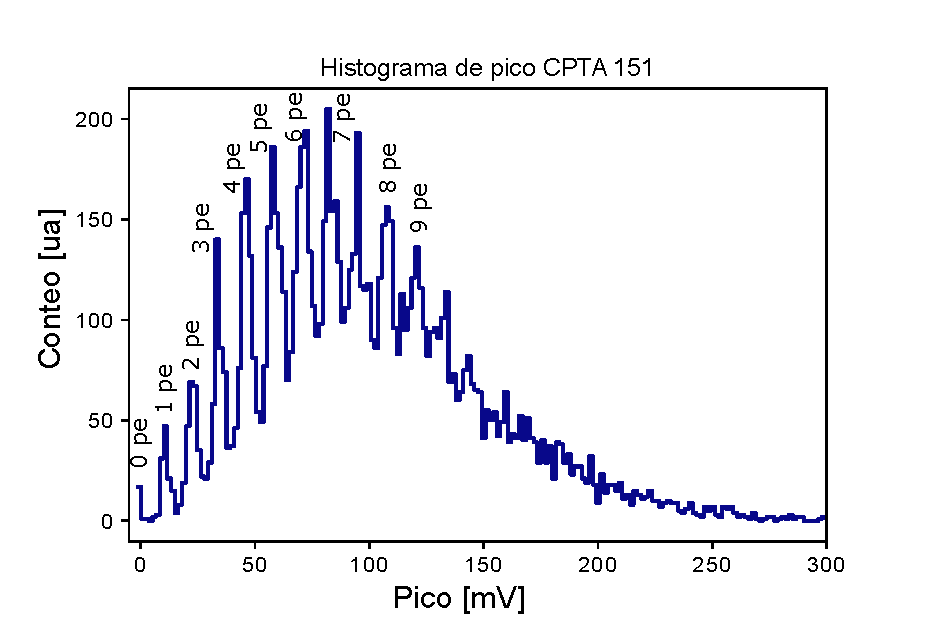
\includegraphics[width=1.1\textwidth]{Images/Peak_CPTA.eps}
         \caption{}
         \label{fig:peak_CPTA}
     \end{subfigure}
        \caption{Forma característica del histograma de pico para los SiPM S13360-1350CS de Hamamatsu (izquierda) y CPTA 151 (derecha). La distancia entre los picos del histograma es constante y determina el equivalente en voltaje de 1 p.e., siendo $13.67~\mbox{mV}$ para el SiPM S13360-1350CS de Hamamatsu y $12.09~\mbox{mV}$ para el CPTA 151.}
        \label{fig:peak}
\end{figure}
\\ \\
Finalmente, en la Fig. \ref{fig:PDF} se muestra la forma de los pulsos de voltaje generados por los eventos para una temperatura de 25 $^\circ$C y unos voltajes de polarización de $56~\mbox{V}$ y $53~\mbox{V}$ para el SiPM de Hamamatsu y CPTA respectivamente. Adicionalmente, se muestra la densidad de probabilidad de la amplitud de estos pulsos, donde se notan zonas más probables que corresponden a la línea base y a los pulsos con una amplitudes que son múltiplos enteros de 1 p.e.  
\begin{figure}[h!]
     \centering
     \begin{subfigure}[b]{0.49\textwidth}
         \centering
         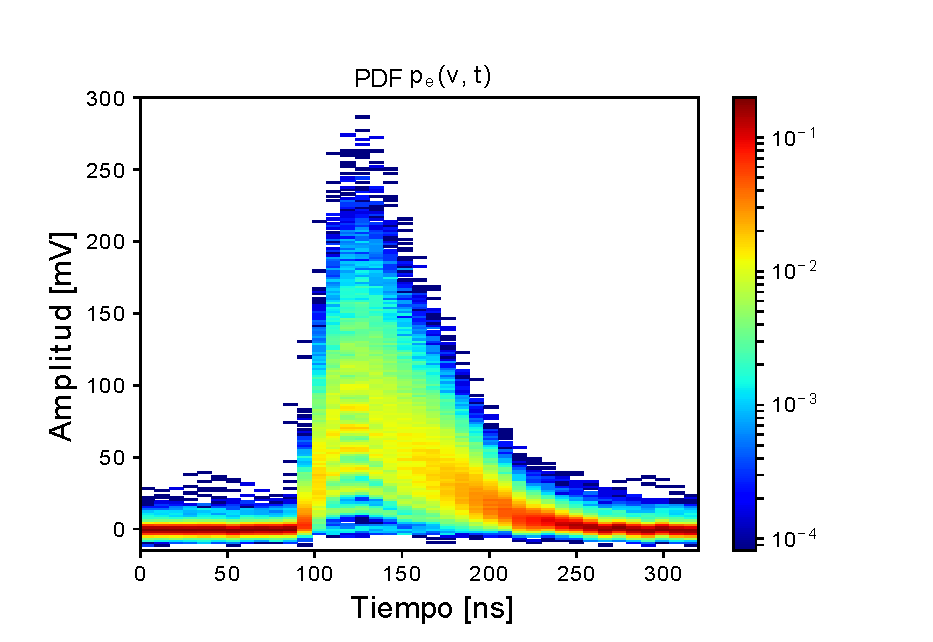
\includegraphics[width=1.1\textwidth]{Images/PDF_1350CS.eps}
         \caption{Hamamatsu S13360-1350CS.}
         \label{fig:PDF_1350CS}
     \end{subfigure}
     %\hfill
     \begin{subfigure}[b]{0.49\textwidth}
         \centering
         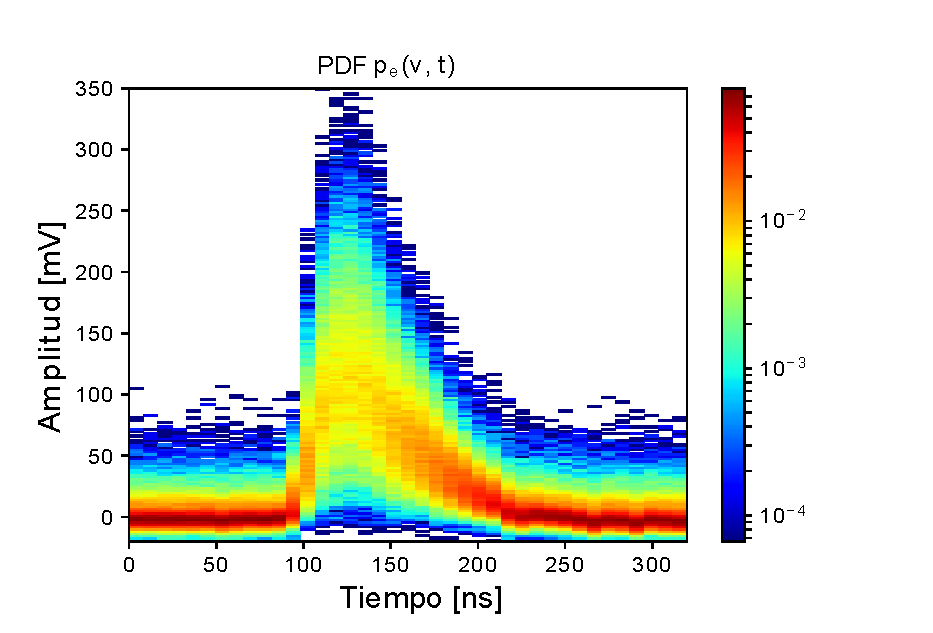
\includegraphics[width=1.1\textwidth]{Images/PDF_CPTA151.eps}
         \caption{CPTA151.}
         \label{fig:PDF_CPTA}
     \end{subfigure}
        \caption{Forma de los pulsos de voltaje generados por los SiPM S13360-1350CS de Hamamatsu (izquierda) y CPTA 151 (derecha) a 25 $^\circ$C y un voltaje de polarización de $56~\mbox{V}$ y $53~\mbox{V}$ respectivamente. Las regiones con una densidad de probabilidad (PDF) mayor corresponden al pedestal y a pulsos con amplitudes que son múltiplos enteros de 1 p.e.}
        \label{fig:PDF}
\end{figure}

\section{Tasa de conteo oscuro}
Para la caracterización de la tasa de conteo oscuro (DCR) en función de la temperatura se utilizó un voltaje de polarización de $56~\mbox{V}$ y $53 ~\mbox{V}$ para el SiPM de Hamamatsu y CPTA respectivamente. Asimismo, el cálculo del DCR para cada una de las temperaturas de estudio se utilizó la expresión \ref{DCR_eq} y su resultado se muestra en la Fig. \ref{fig:DCR_vs_T}, donde se observa que el SiPM de hamamatsu presenta una mayor dependencia de la temperatura en el DCR ($0.85 kHz/ ^\circ$C) con respecto al CPTA ($4.32 Hz/ ^\circ$C). 
\begin{figure}[h!]
     \centering
     \begin{subfigure}[b]{0.49\textwidth}
         \centering
         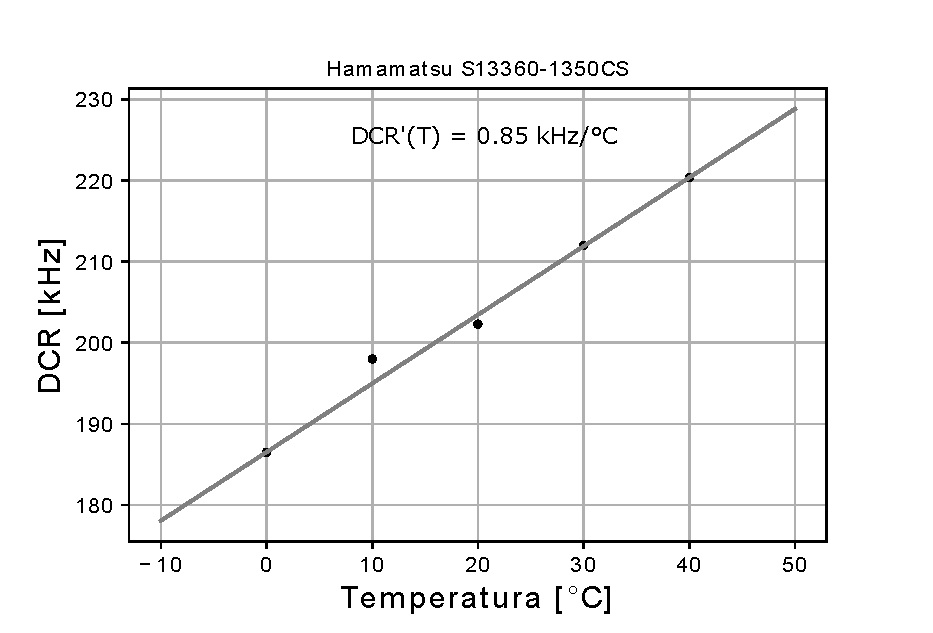
\includegraphics[width=1.1\textwidth]{Images/DCR_T_1350CS.eps}
         \caption{}
         \label{fig:DCR_T_1350CS}
     \end{subfigure}
     %\hfill
     \begin{subfigure}[b]{0.49\textwidth}
         \centering
         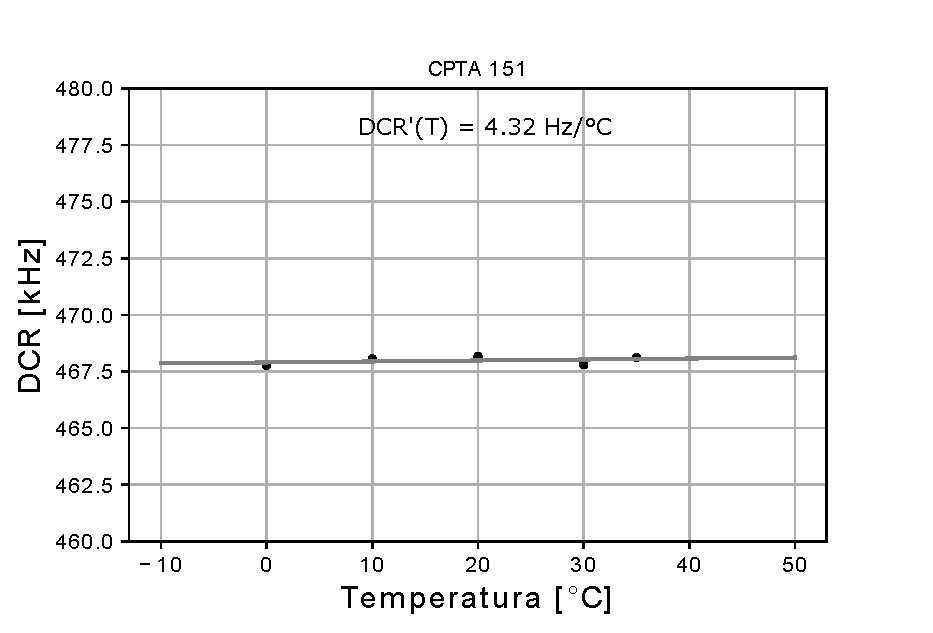
\includegraphics[width=1.1\textwidth]{Images/DCR_T_CPTA.eps}
         \caption{}
         \label{fig:DCR_T_CPTA}
     \end{subfigure}
        \caption{Tasa de conteo oscuro en función de la temperatura para los SiPM S13360-1350CS de Hamamatsu (izquierda) y CPTA 151 (derecha). La razón de cambio del DCR es $0.85 kHz/ ^\circ$C para el SiPM de Hamamatsu y  $4.32 Hz/ ^\circ$C para el CPTA.}
        \label{fig:DCR_vs_T}
\end{figure}
\\ \\
Por otra parte, en la Fig. \ref{fig:DCR_vs_ov} se muestra la dependencia del DCR del sobre-voltaje, en este caso se estableció la temperatura en 25  $^\circ$C y se polarizó  el SiPM de Hamamatsu con $54~\mbox{V}$, $55~\mbox{V}$ y $56~\mbox{V}$ y el CPTA con $51~\mbox{V}$, $52~\mbox{V}$ y $53~\mbox{V}$. Se obtuvo que el cambio del DCR en función del sobre voltaje es $1.1~kHz/V$ para el SiPM de Hamamatsu y $0.35~kHz/V$ para el CPTA.
\begin{figure}[h!]
     \centering
     \begin{subfigure}[b]{0.49\textwidth}
         \centering
         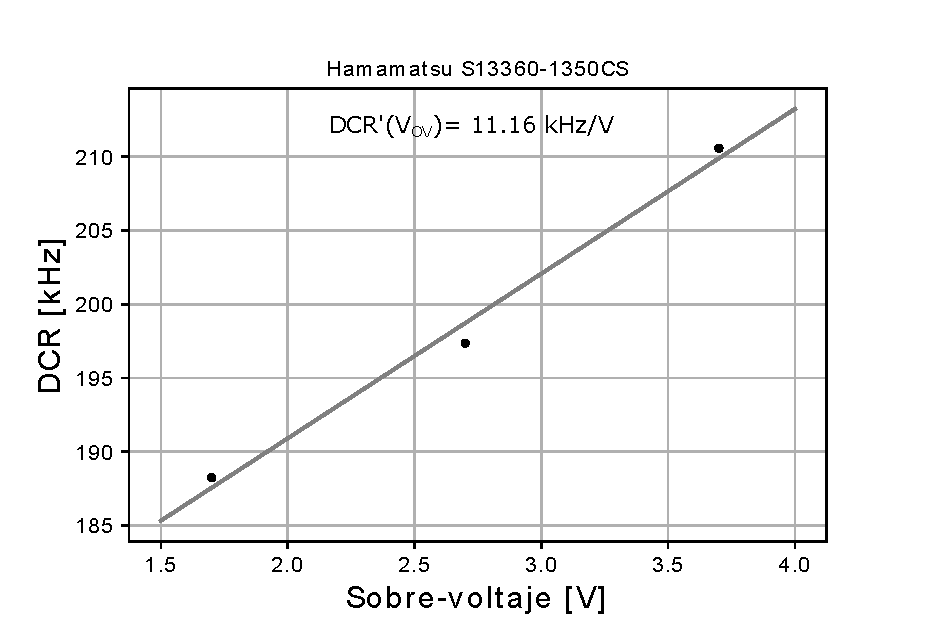
\includegraphics[width=1.1\textwidth]{Images/DCR_vs_ov_1350CS.eps}
         \caption{}
         \label{fig:DCR_ov_1350CS}
     \end{subfigure}
     %\hfill
     \begin{subfigure}[b]{0.49\textwidth}
         \centering
         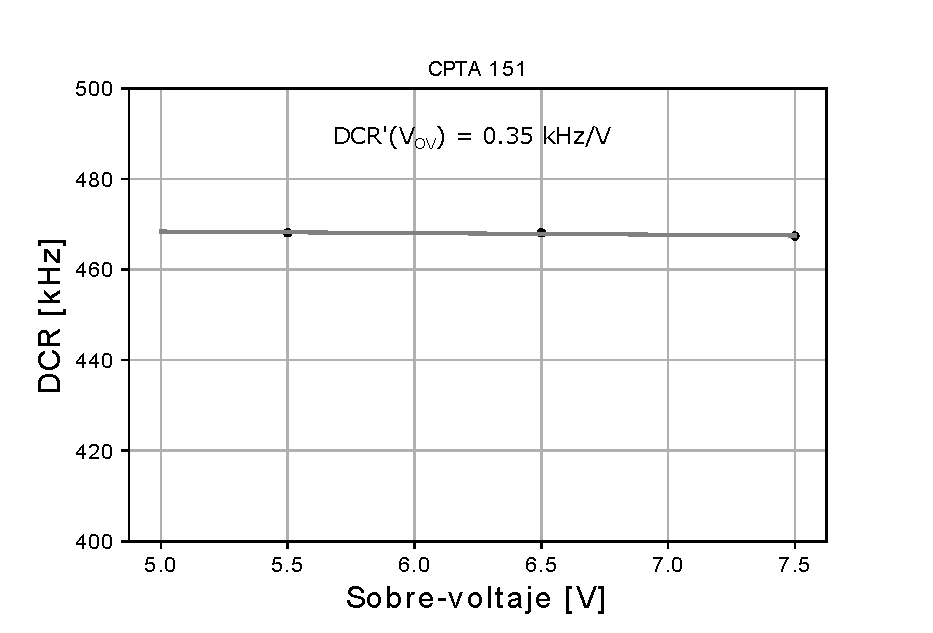
\includegraphics[width=1.1\textwidth]{Images/DCR_vs_ov_CPTA.eps}
         \caption{}
         \label{fig:DCR_ov_CPTA}
     \end{subfigure}
        \caption{Tasa de conteo oscuro en función del sobre-voltaje para los SiPM S13360-1350CS de Hamamatsu (izquierda) y CPTA 151 (derecha). Se puede observar que los cambios en el sobre-voltaje tienen más influencia en el DCR para el SiPM de Hamamatsu que para el CPTA.}
        \label{fig:DCR_vs_ov}
\end{figure}
\\ \\
Finalmente, se establecieron diferentes umbrales en el rango de $0.1$ p.e. a $3.1$ p.e. y se calculó la frecuencia de los eventos que superan estos umbrales para tres voltajes de polarización diferentes, obteniendo la Fig. \ref{fig:DCR_vs_th}, donde se puede observar que para umbrales mayores a 3 p.e. el DCR es menor a 100 Hz.  
\begin{figure}[h!]
     \centering
     \begin{subfigure}[b]{0.49\textwidth}
         \centering
         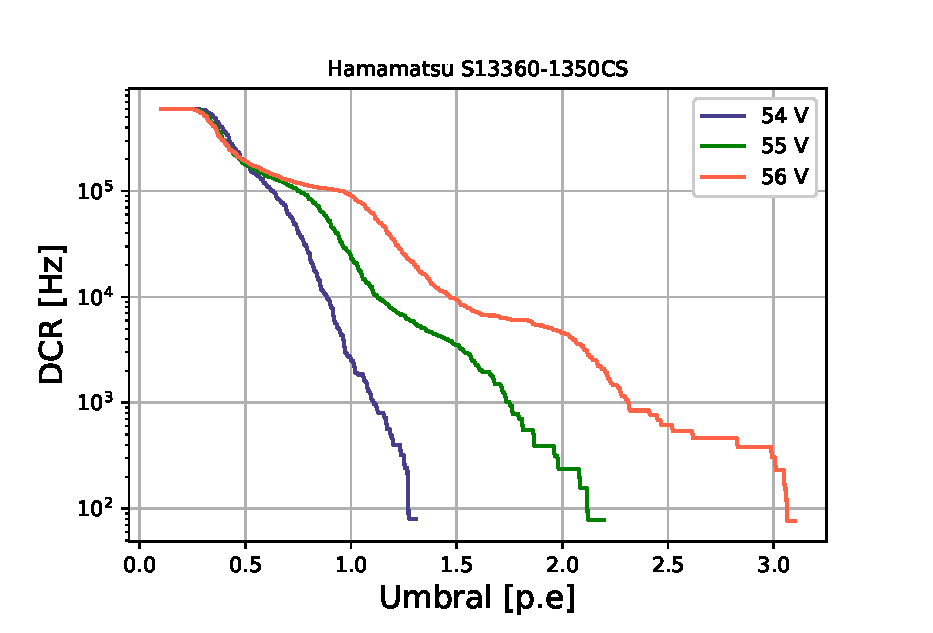
\includegraphics[width=1.1\textwidth]{Images/DCR_vs_th_1350CS.eps}
         \caption{}
         \label{fig:DCR_vs_th_1}
     \end{subfigure}
     %\hfill
     \begin{subfigure}[b]{0.49\textwidth}
         \centering
         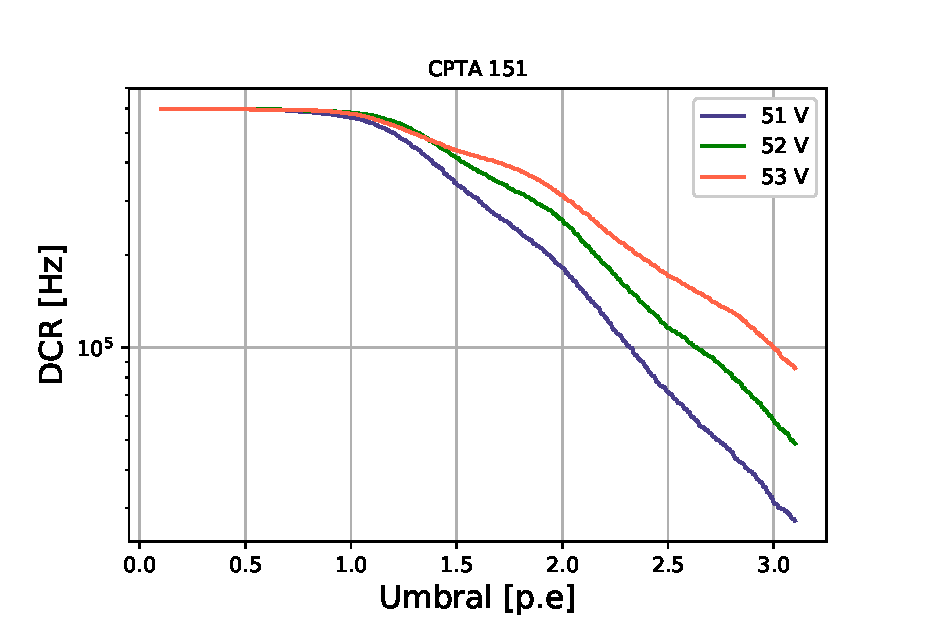
\includegraphics[width=1.1\textwidth]{Images/DCR_vs_th_CPTA.eps}
         \caption{}
         \label{fig:DCR_vs_th_2}
     \end{subfigure}
        \caption{Tasa de conteo oscuro en función de un umbral de $0.1$ p.e. a $3.1$ p.e. para tres voltajes de polarización: 54 V, 55 V y 56 V para el SiPM S13360-1350CS de Hamamatsu (izquierda) y 51 V, 52 V y 53 V para el CPTA 151 (derecha).}
        \label{fig:DCR_vs_th}
\end{figure}
\section{Crosstalk y Afterpulses}
Para calcular de la probabilidad del \textit{crosstalk} y  \textit{afterpulses} se estableció la temperatura a 25 $^\circ$C y el voltaje de polarización a  $56~\mbox{V}$ para el SiPM de Hamamatsu y $53~\mbox{V}$ para el CPTA. En la Fig. \ref{fig:NoiseP} se muestra un conjunto de 150 pulsos, cada pulso es dividido en tres partes, antes, durante y después de la estimulación. Estas ventanas de tiempo se utilizan en las expresiones \ref{CT_eq} y \ref{AP_eq} para realizar el cálculo \textit{crosstalk} y  \textit{afterpulses}. En la tabla \ref{AP_CT} se muestra la probabilidad de los ruidos correlacionados, siendo más alta la probabilidad de  \textit{crosstalk} y  \textit{afterpulses} en SiPM CPTA 151.   
\begin{figure}[h!]
\begin{centering}
  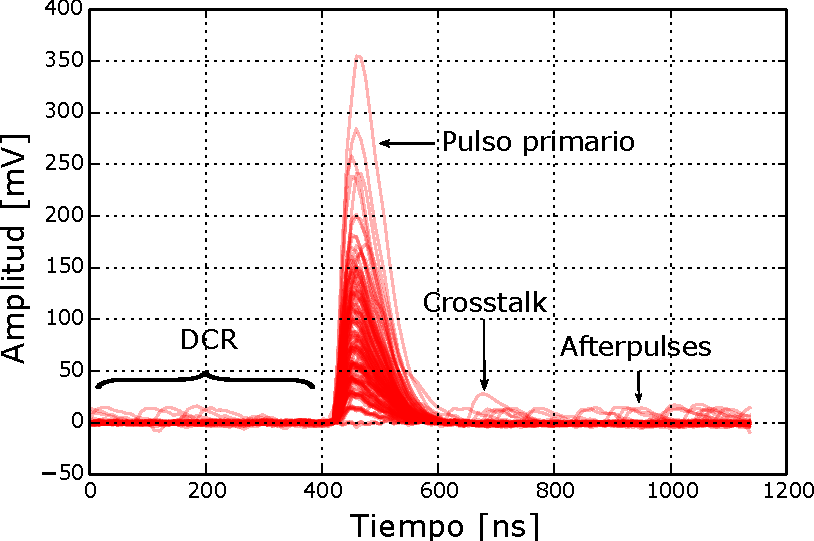
\includegraphics[width=0.7\textwidth]{Images/100P_1350CS.pdf}
  \caption{Pulsos característicos de DCR, \textit{crosstalk} y \textit{afterpulses} antes y después del pulso primario.}
  \label{fig:NoiseP}
  \par\end{centering}
\end{figure}
\begin{table}[h!]
\caption{Probabilidad del ruido correlacionado para 25 $^\circ$C a un voltaje de polarización de 56 V para el SiPM S13360-1350CS de Hamamatsu y 53 V para el CPTA 151.}
    \label{AP_CT}
	\centering
%    \begin{threeparttable}
	\begin{tabular}{ c  c  c}
    \hline
    SiPM       & Hamamatsu S13360-1350CS  & CPTA 151      \\ \hline
    \multicolumn{1}{l}{\textit{Crosstalk}[\%] }     &   $5.1$      & $ 19.1$ \\
%    \multicolumn{1}{l}{\textit{Crosstalk}[kHz]}      &  $5.9$       & $89.4$ \\
    \multicolumn{1}{l}{\textit{Afterpulses}[\%]}      & $2.78$         & $3.08$ \\
%    \multicolumn{1}{l}{\textit{Afterpulses}[kHz]}      & $13.05$         & $14.4$  \\ \hline
	\end{tabular}	
\end{table}
\\ \\
Por último, en la Fig.\ref{fig:Noise_vs_Ov}. se muestra la probabilidad de \textit{crosstalk} y  \textit{afterpulses} en función del sobre-voltaje a una temperatura de 25 $^\circ$C para el SiPM S13360-1350CS de Hamamatsu, se puede observar una relación exponencial que permite concluir que en términos del ruido correlacionado no es recomendable utilizar el SiPM con un sobre-voltaje mayor a $3.7$ V.

\begin{figure}[ht!]
     \centering
     \begin{subfigure}[b]{0.49\textwidth}
         \centering
         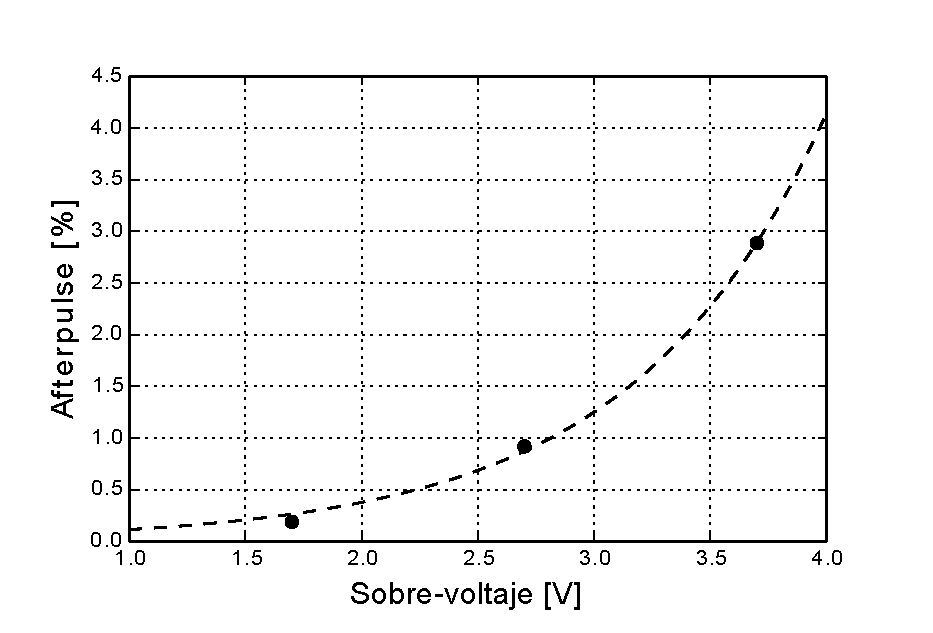
\includegraphics[width=1.1\textwidth]{Images/After_vs_Ov_1350CS.eps}
         \caption{}
         \label{fig:After_vs_Ov}
     \end{subfigure}
     %\hfill
     \begin{subfigure}[b]{0.49\textwidth}
         \centering
         \includegraphics[width=1.1\textwidth]{Images/Cross_vs_Ov_1350CS.eps}
         \caption{}
         \label{fig:Cross_vs_Ov}
     \end{subfigure}
        \caption{Probabilidad de \textit{afterpulse} (izquierda) y \textit{crosstalk} (derecha) para sobre voltajes de $1.7$ V, $2.7$ V y $3.7$ V para el SiPM S13360-1350CS de Hamamatsu.}
        \label{fig:Noise_vs_Ov}
\end{figure}